% !TeX root=main.tex

\chapter{کارهای مرتبط} \label{ch:related}
\thispagestyle{empty}


\section{مقدمه}
\label{sec:intro}
\paragraph{}
{
    در این فصل به معرفی کارهای مشابه و شرح
    رویکردهای مورد استفاده برای حل مساله‌ی 
    کنترل و پایش دستگاه‌های اینترنت اشیاء بر بستر کوبرنیتز می‌پردازیم.    
}

\section{
    روش‌های متفاوت حل مسئله کنترل و پایش دستگاه‌های اینترنت اشیاء
}
\label{sec:approaches_to_monitoring_iot}
\paragraph{}{
    در مسئله مورد بحث، کارهای زیادی انجام نشده است. در ادامه به بررسی برخی از معدود روش‌های حل این مسئله می‌پردازیم
}
\subsection{
    کنترل و پایش دستگاه‌های اینترنت اشیاء بر پایه زنجیره‌ی بلوکی
}
\label{sec:blockchain_based_monitoring}
\paragraph{}{
    در \cite{s19040856}،
    نویسندگان به بررسی مسائل مدیریت و نظارت بر دستگاه‌های اینترنت اشیاء می‌پردازند
    و از تکنولوژی زنجیره‌ی بلوکی\footnote{\lr{Blockchain}} برای حل این مسائل استفاده می‌کنند. 
    در این مقاله، نویسندگان نکاتی را در مورد مزایا و چالش‌های استفاده از زنجیره‌ی بلوکی در مدیریت 
    و نظارت بر دستگاه‌های اینترنت اشیاء بررسی می‌کنند. آنها به بررسی معماری زنجیره‌ی بلوکی و
    نحوه استفاده آن در این زمینه می‌پردازند. همچنین، روش‌های مختلف برای اعتبارسنجی و امنیت 
    دستگاه‌های اینترنت اشیاء با استفاده از زنجیره‌ی بلوکی را مورد بررسی قرار می‌دهند. در ادامه، 
    نویسندگان به بررسی موارد کاربردی مدیریت و نظارت بر دستگاه‌های اینترنت اشیاء با استفاده
    از زنجیره‌ی بلوکی می‌پردازند. آنها به بررسی روش‌هایی برای ثبت و ذخیره داده‌های مربوط به 
    دستگاه‌های اینترنت اشیاء در زنجیره‌ی بلوکی می‌پردازند و نحوه استفاده از قراردادهای هوشمند
    برای اجرای منطق کسب و کار را بررسی می‌کنند.
    \begin{figure}[H]
        \center{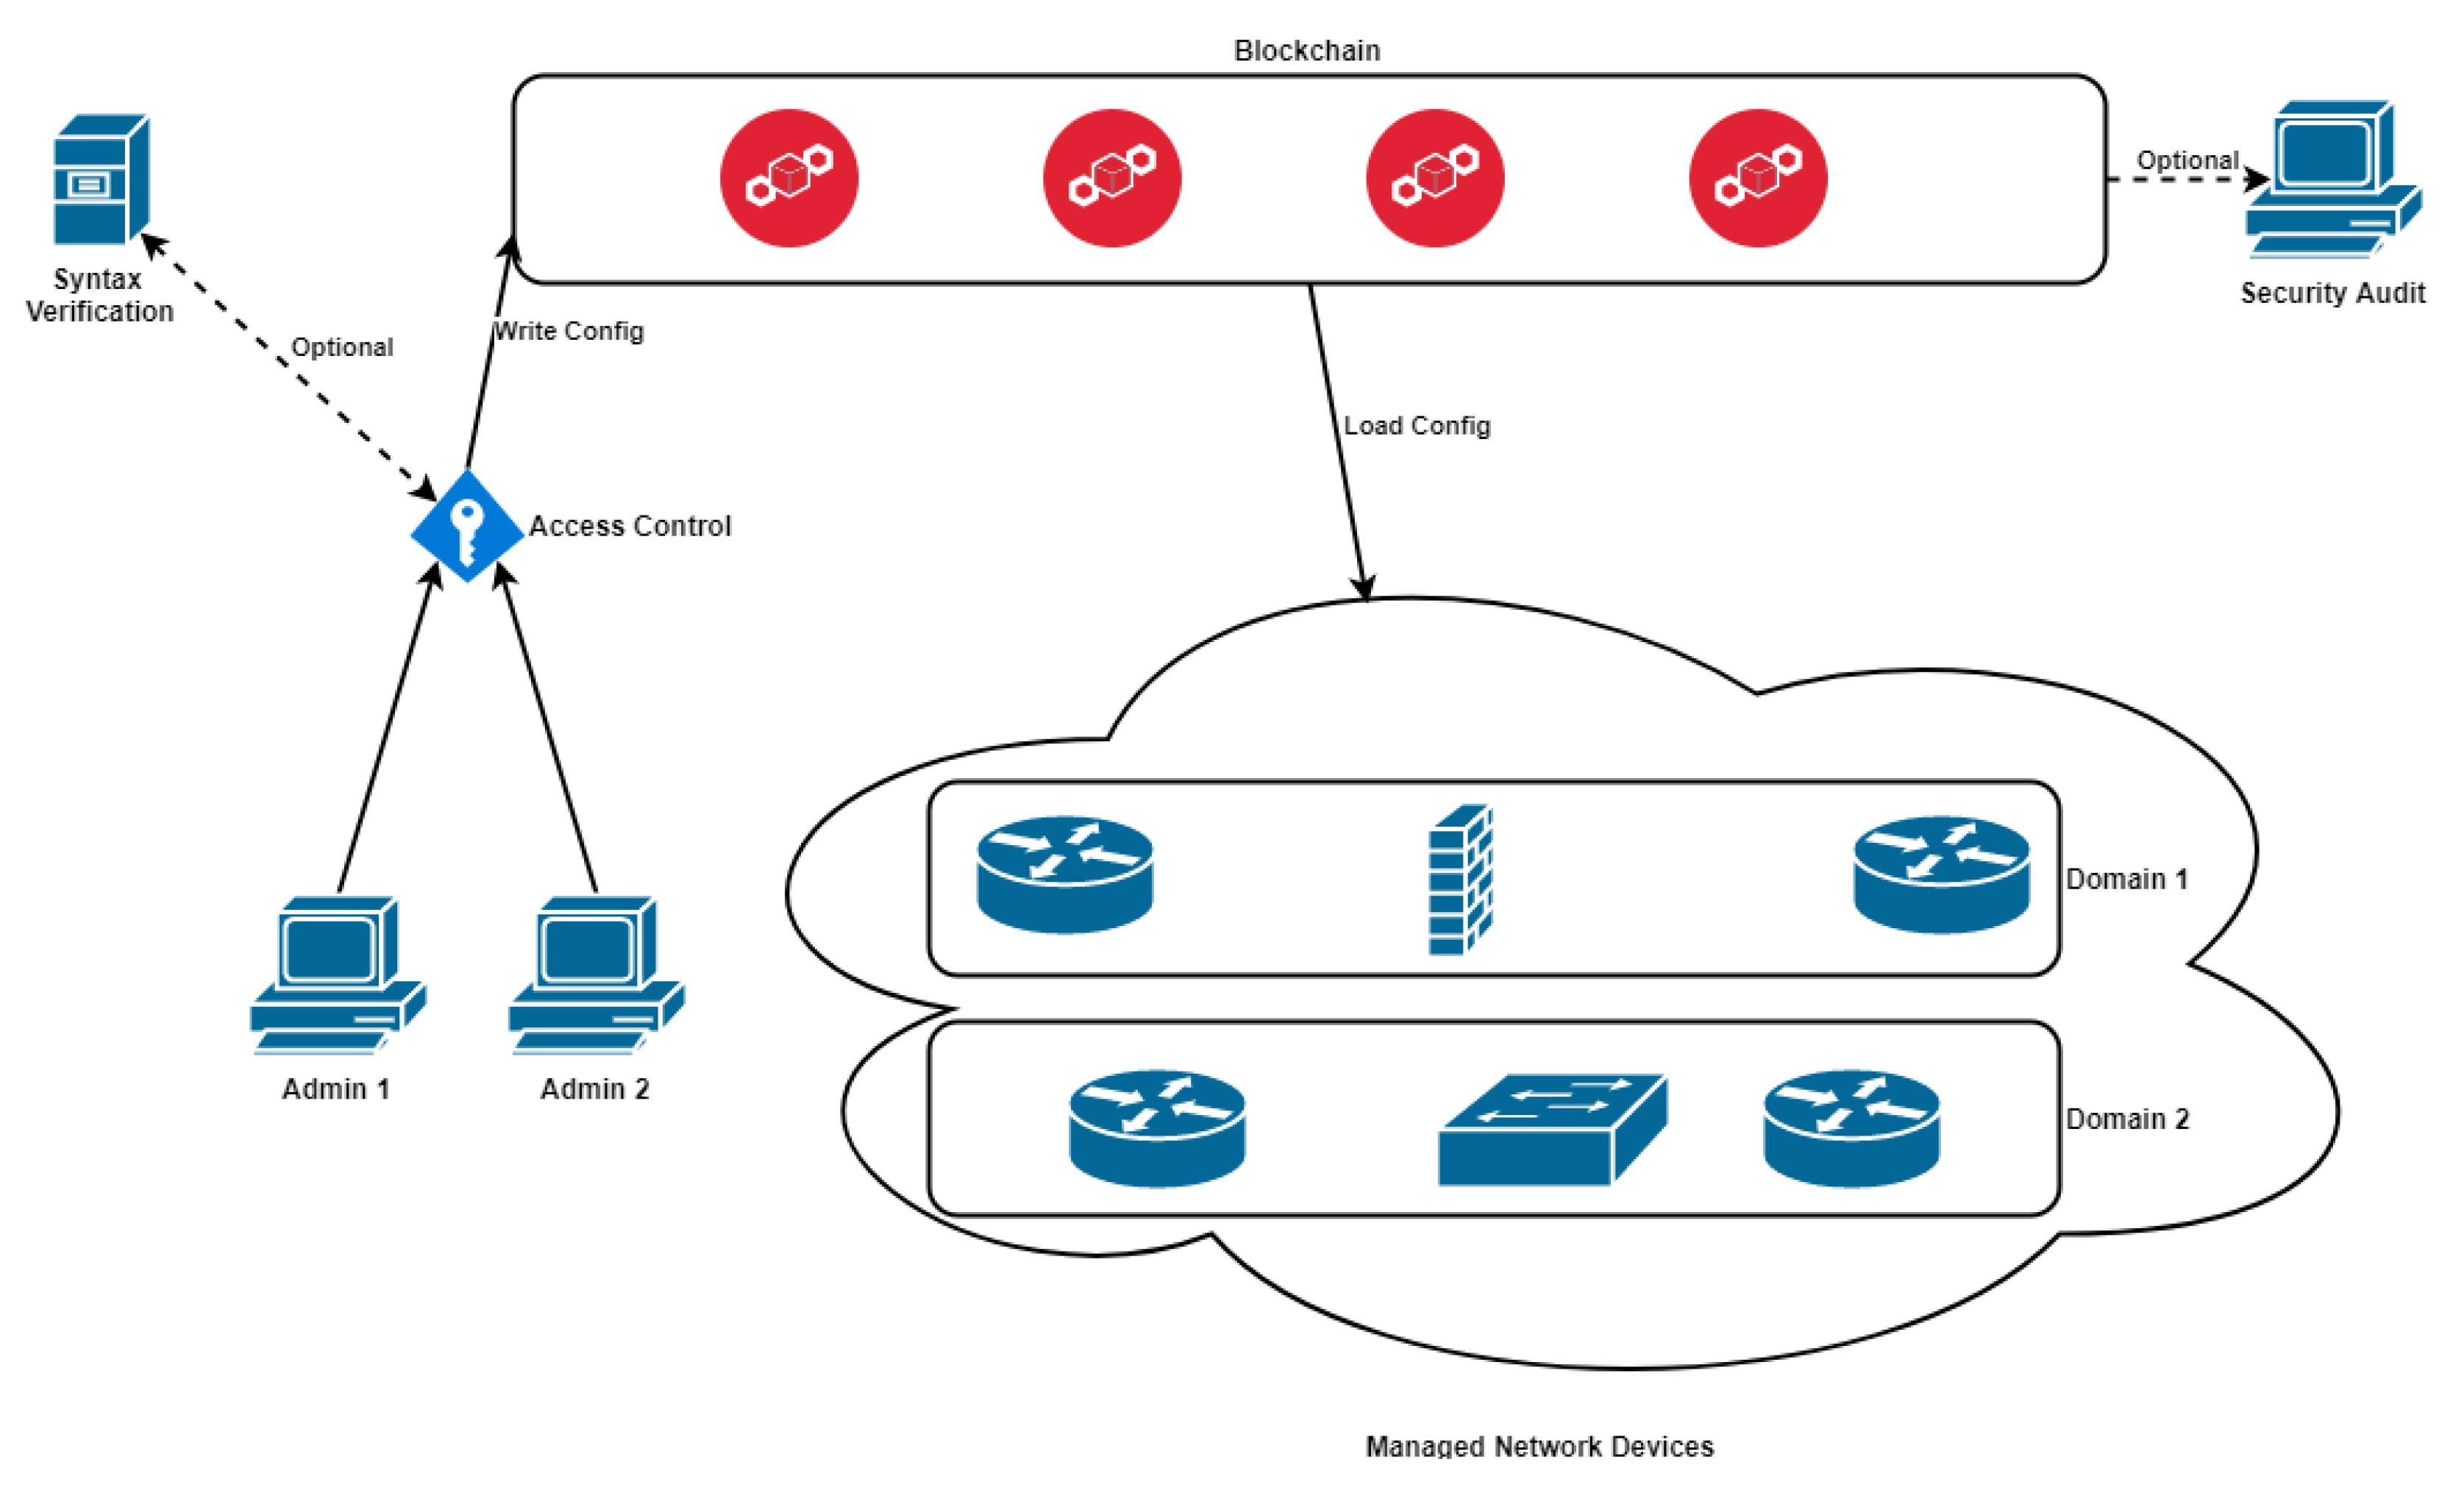
\includegraphics[width=\textwidth]{figs/ref_figs/blockchain_monitoring.png}}
        \caption{پایش مبتنی بر زنجیره‌ی بلوکی \cite{s19040856}}
        \label{fig:blockchain_monitoring}
    \end{figure}
}

\subsection{
    گسترش کوبرنیتز بر روی دستگا‌های لبه
}
\label{subsec:extending_kubernetes_to_edge}
\paragraph{}{
    در \cite{exteing-kubernetes-to-low-resource-edge-devices}،
    نویسندگان به بررسی نیازمندی‌های موجود برای ارتقاء خوشه‌های کوبرنیتز به دستگاه‌های لبه
    با منابع کم می‌پردازند و نشان می‌دهند که استفاده از کوبلت مجازی می‌تواند یک راه حل
    مناسب برای این امر باشد. آنها به توضیح عملکرد کوبلت مجازی، که نماینده‌های مجازی در
    خوشه کوبرنیتز است، می‌پردازند و نحوه تعامل آن با دستگاه‌های لبه را تشریح می‌کنند. در
    ادامه، نویسندگان به بررسی فناوری‌ها و پروتکل‌های مورد استفاده در کوبلت مجازی می‌پردازند
    و نحوه اتصال و مدیریت آن را توضیح می‌دهند. آنها به بررسی عملکرد استفاده از کوبلت مجازی 
    در دستگاه‌های لبه، می‌پردازند. در نهایت، نویسندگان به ارزیابی و ارائه نتایج آزمایش‌هایی
    که در ارتقاء خوشه‌های کوبرنیتز به دستگاه‌های لبه با استفاده از کوبلت مجازی انجام
    شده است، می‌پردازند. آنها به بررسی کارایی و کارایی سیستم، زمان پاسخ و نیازمندی‌های 
    منابع مورد نیاز برای استفاده از کوبلت مجازی در دستگاه‌های لبه می‌پردازند.
}

\subsection{
    پایش خانه هوشمند به کمک دستگاه‌های اینترنت اشیاء
}
\label{subsec:iot_based_monitoring}
\paragraph{}{
    در \cite{iot_based_monitoring}،
    نویسندگان به بررسی مزایا و چالش‌های استفاده از اینترنت اشیاء در خانه‌های هوشمند می‌پردازند.
    آنها به تشریح معماری سیستم نظارت و کنترل مبتنی بر اینترنت اشیاء برای خودکارسازی خانه
    می‌پردازند و نحوه ارتباط و تعامل بین اجزای مختلف این سیستم را بررسی می‌کنند. در ادامه، 
    نویسندگان به توضیح کارکردها و قابلیت‌های سیستم نظارت و کنترل مبتنی بر اینترنت اشیاء برای
    خودکارسازی خانه می‌پردازند. آنها به بررسی امکانات نظارت بر دستگاه‌های خانگی، کنترل سیستم‌های 
    روشنایی و الکترونیکی، کنترل دما و رطوبت، و همچنین مدیریت از راه دور این سیستم می‌پردازند. 
    در نهایت، نویسندگان به ارائه نتایج واقعی سیستم نظارت و کنترل مبتنی بر اینترنت اشیاء برای 
    خودکارسازی خانه پرداخته و مورد استفاده قرار گرفتن این سیستم را بررسی می‌کنند. آنها به تأثیر
    این سیستم بر کاهش مصرف انرژی، راحتی کاربران و بهبود کیفیت زندگی در خانه اشاره می‌کنند.
}

\subsection{
    پایش دستگاه‌های اینترنت اشیاء بر پایه کوبرنیتز
}
\label{subsec:iot_device_management}
\paragraph{}{‍
    در این مقاله \cite{Mlynka2022thesis}، چالش‌های فناوریکی در توسعه معماری اینترنت اشیاء بررسی می‌شود و راه‌حلی خاص بر بستر کوبرنیتز برای مدیریت میلیون‌ها دستگاه در محیط‌های مختلف پیشنهاد می‌شود. این پایان‌نامه بر تأسیس یک زیرساخت اینترنت اشیاء کامل با استفاده از ابزار کوبرنیتز تمرکز دارد که به عنوان یکی از بهترین راه‌حل‌ها برای کنترل منابع مختلف شناخته شده است و در محیط‌های ابری به‌طور گسترده برای مدیریت بارکاری نرم‌افزاری استفاده می‌شود. هدف اصلی این کار، ایجاد یک معماری اینترنت اشیاء انعطاف‌پذیر، مقیاس‌پذیر و گسترش‌پذیر با تأکید بر امنیت در تمام لایه‌های آن است. مقاله نیز به بررسی فناوری‌های موردنیاز برای استفاده از کوبرنیتز در طراحی معماری اینترنت اشیاء می‌پردازد و تکنولوژی‌های مرتبط دیگری را نیز معرفی می‌کند که به هدف‌های مشخص شده در این تحقیق منطبق هستند.
    \begin{figure}[H]
        \center{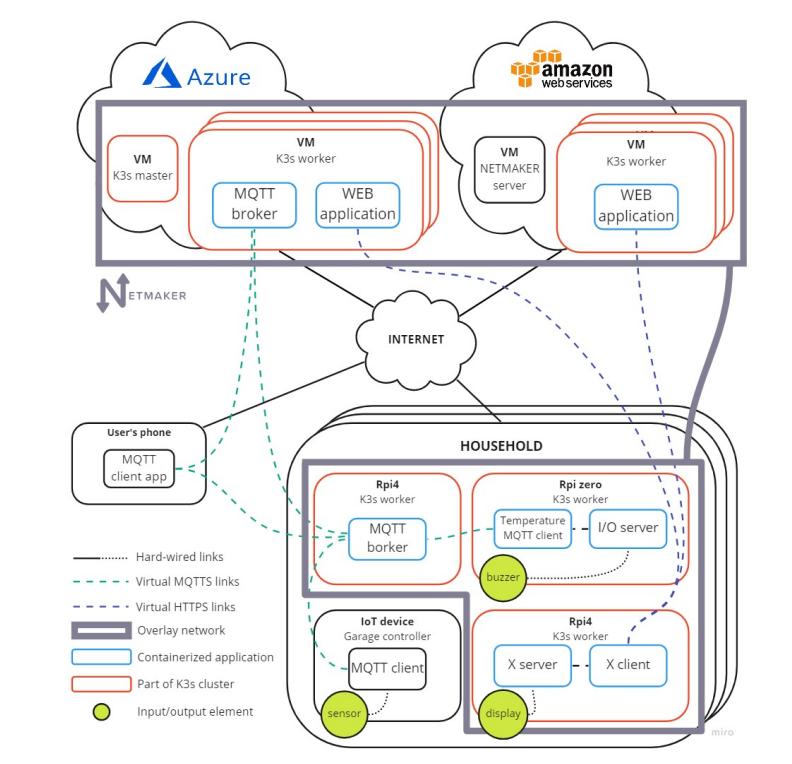
\includegraphics[width=\textwidth]{figs/ref_figs/iot_monitoring.png}}
        \caption{پایش مبتنی بر کوبرنیتز \cite{Mlynka2022thesis}}
        \label{fig:iot_monitoring}
    \end{figure}
‍}